\subsection{Введение}
В данной части лабораторной работы произведено исследование и анализ частотных характеристик RCL-цепи с последовательным и параллельным подключениями ветвей с индуктивным и ёмкостным элементами соответственно.

\subsection{Параметры элементов исследуемых схем}
\begin{center}
	Известные значения:
	\[
		\begin{gathered}
			U_{\text{д}} = 6 \, \text{В}, \psi_{\text{н}} = -150^{\circ}, R_1 = 17 \, \text{Ом}, R_k = 5 \, \text{Ом} \\
			L_k = 23.094 \, \text{мГн}, C = 71.454 \, \text{мкФ}
		\end{gathered}
	\]
\end{center}

% -------------------------------

\subsection{Двухполюсник 6}

\subsubsection{Схема исследуемой цепи}
\begin{figure}[H]
	\centering
	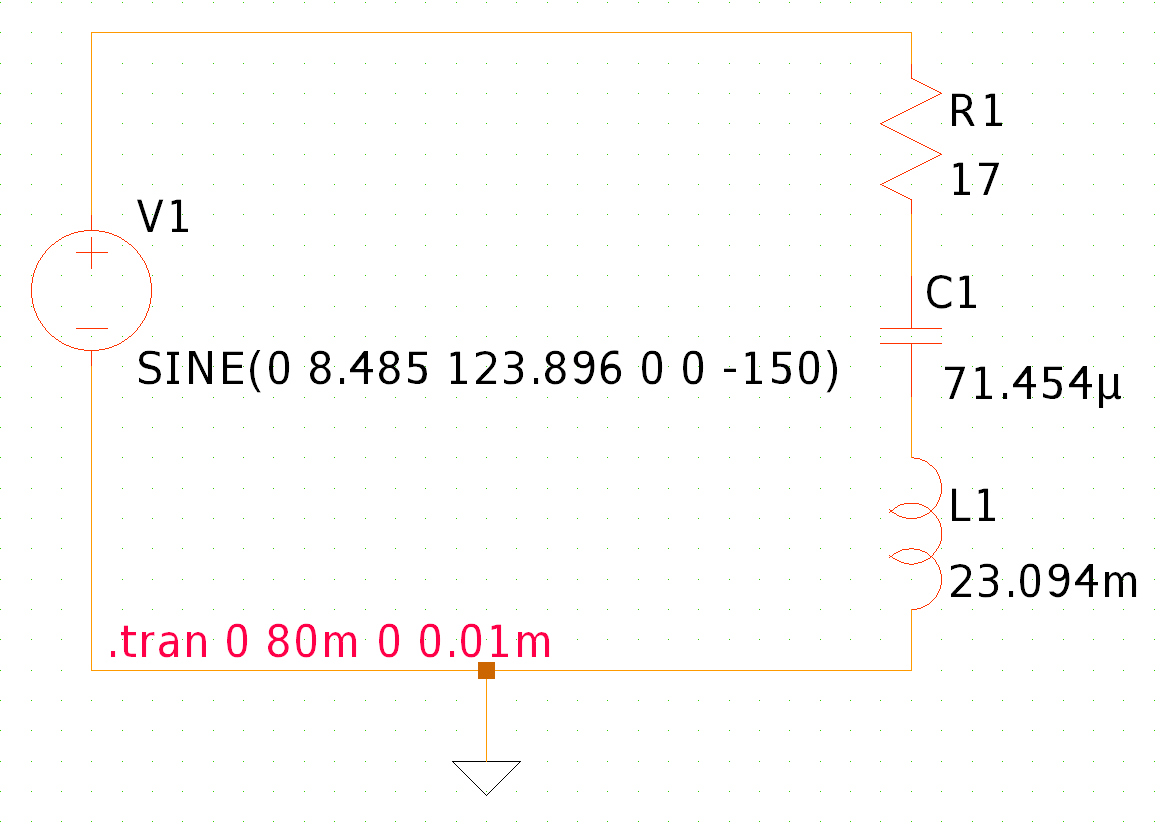
\includegraphics[width=0.65\textwidth]{./data/schema1_p2}
	\caption{Схема замещения Двухполюсника 6 (в резонансе) в LTspice.}
\end{figure}

\subsubsection{Расчётные формулы и расчёты}
\begin{enumerate}
	\item Резонансная частота:

	      \[
		      f_0 = \frac{1}{2 \cdot \pi \cdot \sqrt{L \cdot C}} = \frac{1}{2 \cdot \pi \cdot \sqrt{23.094 \cdot 71.454 \cdot 10^{-3} \cdot 10^{-6}}} = 123.896 \, \text{Гц}
	      \]

	\item Угловая частота:

	      \[
		      \omega = 2 \cdot \pi \cdot f
	      \]

	\item Действующий ток в цепи:

	      \[
		      I = \frac{U_\text{д}}{\sqrt{(R_1+R_k)^2+(\omega L - \frac{1}{\omega C})^2}}
	      \]
	\item Напряжение на резистивном элементе:

	      \[
		      U_{R_k} = I \cdot R_1
	      \]

	\item Напряжение на индуктивном элементе:

	      \[
		      U_k = I \cdot \sqrt{R_k^2 + (\omega L)^2}
	      \]

	\item Напряжение на ёмкостном элементе:

	      \[
		      U_C = \frac{I}{\omega C}
	      \]

	\item Фазовый сдвиг между входным напряжением и током:

	      \[
		      \phi = \arctan \left(\frac{\omega L - \frac{1}{\omega C}}{R_1 + R_k}\right)
	      \]

	\item Добротность контура:

	      \[
		      \begin{gathered}
			      Q_p = \frac{p}{R_1+R_k} \\
			      \\
			      Q_e = \frac{U_{C_0}}{U_{\text{д}}}
		      \end{gathered}
	      \]

\end{enumerate}


\subsubsection{Заполненная таблица 2.3}
Изменяя частоту источника в диапазоне от $0.1 \cdot f_0$ до $2 \cdot f_0$ были рассчитаны значения по вышеуказанным формулам, а также сняты показания с двухполюсника для указанных частот.

Значения действующего тока в цепи и напряжений на резистивном, ёмкостном и индуктивном элементах были найдены как максимальное измеренное значение ($I_m, U_m$), поделённое на \(\sqrt{2}\) для преобразования амплитудного значения, в действующее.

Фазовый сдвиг вычислен как дельта между синусоидами тока и напряжения при переходе от отрицательных значений к положительным, поделённая на амплитуду напряжения: \( \phi = 180^{\circ} \cdot \frac{\delta h}{h}\).

\begin{table}[H]
	\captionsetup{labelformat=empty}
	\centering
	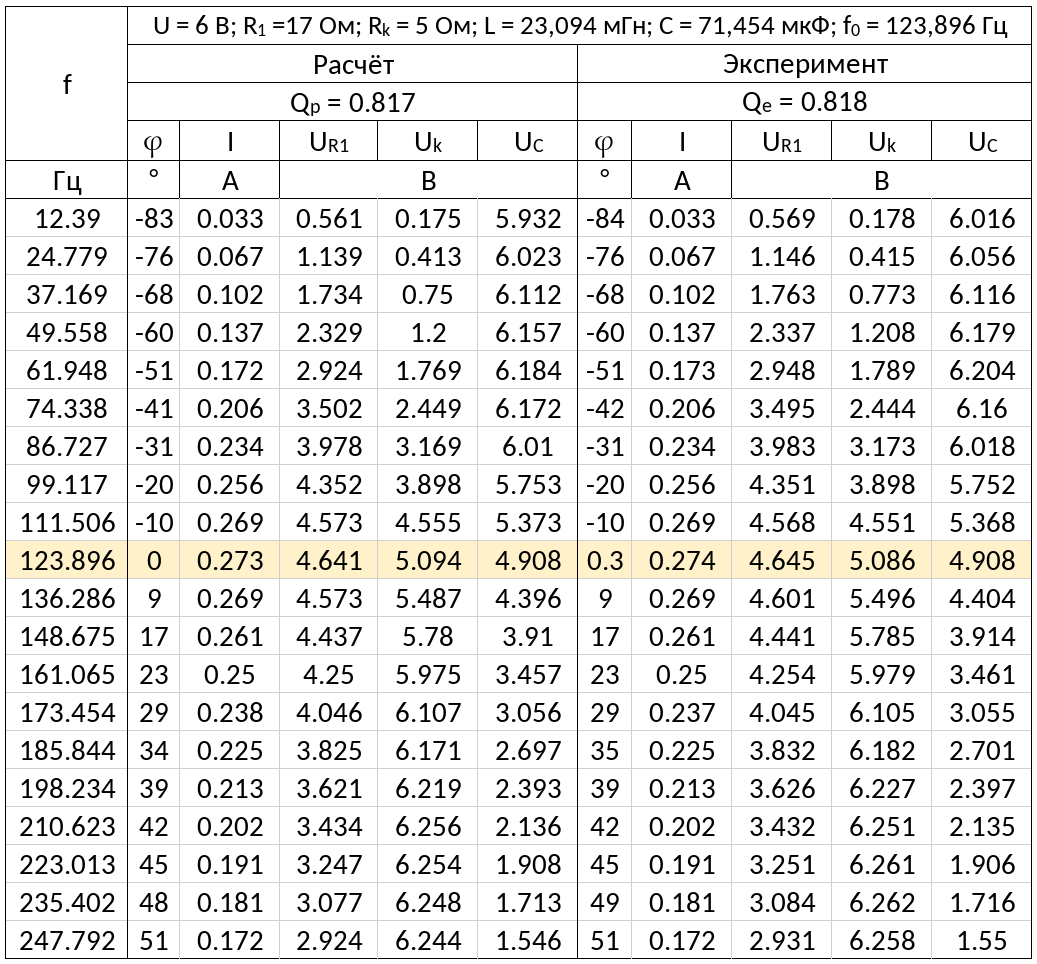
\includegraphics[width=1\textwidth]{./data/table_2-3.png}
	\caption{Итоговая таблица 2.3}
\end{table}


\subsubsection{Графики характеристических зависимостей от частоты}

Графики зависимостей $I(f), \phi(f), U_{R_1} (f), U_k (f), U_C (f)$ поделены на два для большей наглядности и удобства разрешения масштаба - первый показывает зависимости характеристик $I(f), \phi(f)$, второй - $U_{R_1} (f), U_k (f), U_C (f)$.

\begin{figure}[H]
	\centering
	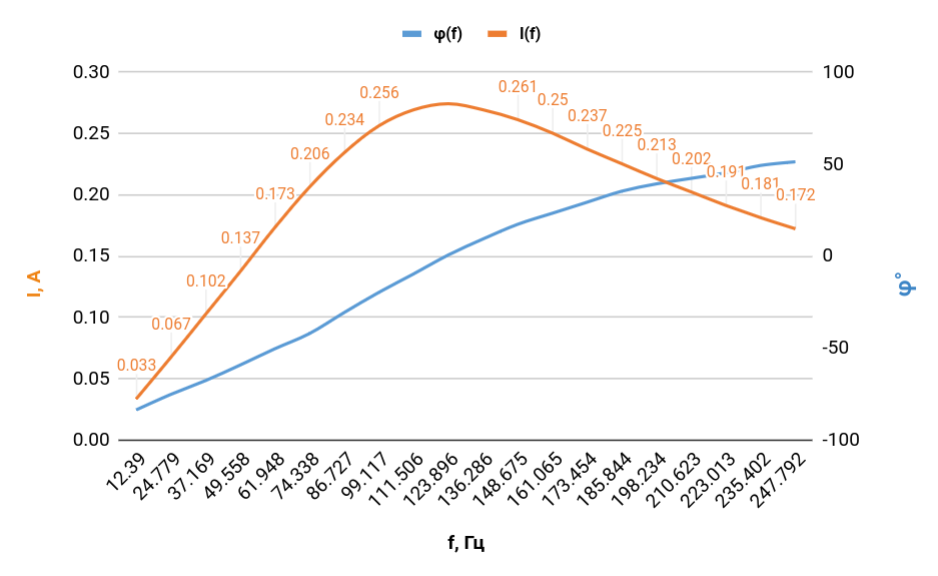
\includegraphics[width=0.95\textwidth]{./data/graph_part2_1.png}
	\caption{Зависимость действующего тока и фазового сдвига от частоты}
\end{figure}

\begin{figure}[H]
	\centering
	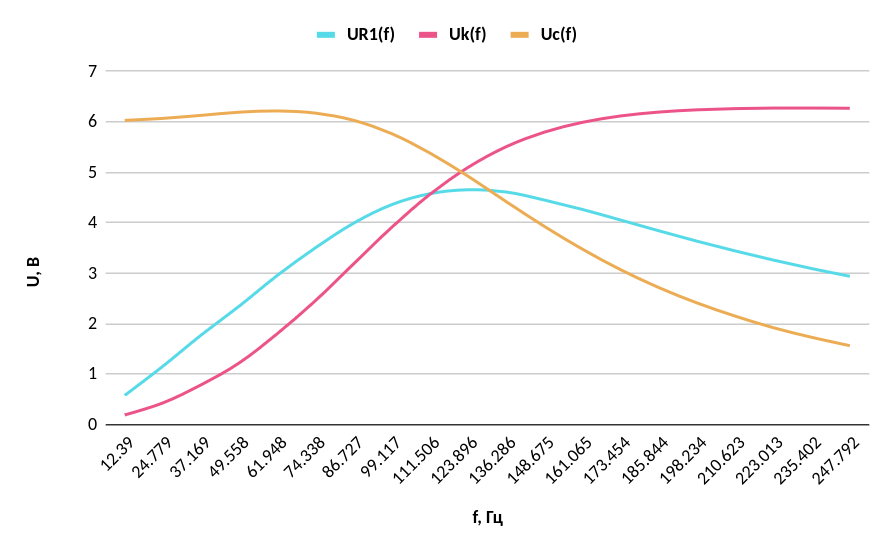
\includegraphics[width=0.95\textwidth]{./data/graph_part2_2.png}
	\caption{Зависимость действующих напряжений от частоты}
\end{figure}


\subsubsection{Векторная диаграмма для состояния резонанса}
Векторная диаграмма, представленная ниже, должна эксперементально подтверждать II Закон Кирхгофа для нашего двухполюсника:

\[
	U_{R_1} + U_k + U_C = U
\]

Диаграмма выполнена в масштабе, 1 клетка = 1 Вольт. По-хорошему, векторы напряжений на катушке и конденсаторе должны компенсировать друг друга в резонансе, но мы специально собрали схему так, что между индуктивным и ёмкостным элементом есть резистивный элемент, в данном случае на 5 Ом, так что можно наглядно сложить векторы и напряжений и получить действующее напряжение в цепи.

Для построения векторной диаграммы рассчитаю фазовые сдвиги действующих напряжений на элементах в момента резонанса:

\[
	\begin{gathered}
		\phi(U_{R_1}) = \psi = -150^\circ \\
		\vspace*{-0.3cm} \\
		\phi(U_{C_1} \, \hat{} \,\, U_{R_1}) = 180^\circ \cdot \frac{\delta h}{h} = 180^\circ \cdot \frac{29.595 - 27.577}{31.606-27.574} = 90.089^\circ \\
		\vspace*{-0.3cm} \\
		\phi(U_{L_1} \, \hat{} \,\, U_{R_1}) = 180^\circ \cdot \frac{\delta h}{h} = 180^\circ \cdot \frac{43.722 - 42.052}{31.606 - 27.274} = -69.39^\circ \, (U_{R_1} \, \text{опережает} \, U_{L_1})\\
		\vspace*{0.4cm} \\
	\end{gathered}
\]

\setlength{\columnsep}{0.5cm}

\begin{multicols}{2}

	\begin{figure}[H]
		\centering
		\begin{tikzpicture}[scale=0.7]

			% Draw the grid
			\draw[very thin, gray] (-6,-6) grid (6,6);

			% Draw the axes
			\draw[-] (-6,0) -- (6,0) node[right];
			\draw[-] (0,-6) -- (0,6) node[above];

			% Draw the current vector (red) with a phase shift of -75 degrees
			\draw[->, red, thick] (0,0) -- ({4.645*cos(-150)}, {4.645*sin(-150)})
			node[end, above left] {$U_{R_1}$};

			% Draw the current vector (red) with a phase shift of -75 degrees
			\draw[->, orange, thick] (0,0) -- ({4.908*cos(-60)}, {4.908*sin(-60)})
			node[end, above left] {$U_{C_1}$};

			% Draw the current vector (red) with a phase shift of -75 degrees
			\draw[->, teal, thick] (0,0) -- ({5.086*cos(-219.39)}, {5.086*sin(-219.39)})
			node[end, above left] {$U_{L_1}$};

			% Labels for the axis
			\node[below left] at (0,0) {$0$};

		\end{tikzpicture}
	\end{figure}

	\columnbreak

	\begin{figure}[H]
		\centering
		\begin{tikzpicture}[scale=0.7]

			% Draw the grid
			\draw[very thin, gray] (-8,-6) grid (4,6);

			% Draw the axes
			\draw[-] (-8,0) -- (4,0) node[right];
			\draw[-] (0,-6) -- (0,6) node[above];

			% Draw the current vector (red) with a phase shift of -75 degrees
			\draw[->, red, thick] ({5.086*cos(-219.39) + 4.8*cos(-60)},{5.086*sin(-219.39) + 4.8*sin(-60)}) -- ({5.086*cos(-219.39) + 4.8*cos(-60) + 4.645*cos(-150)}, {5.086*sin(-219.39) + 4.8*sin(-60) + 4.645*sin(-150)})
			node[end, above left] {$U_{R_1}$};

			% Draw the current vector (red) with a phase shift of -75 degrees
			\draw[->, orange, thick] ({5.086*cos(-219.39)}, {5.086*sin(-219.39)}) -- ({5.086*cos(-219.39) + 4.8*cos(-60)}, {5.086*sin(-219.39) + 4.8*sin(-60)})
			node[end, above left] {$U_{C_1}$};

			% Draw the current vector (red) with a phase shift of -75 degrees
			\draw[->, teal, thick] (0,0) -- ({5.086*cos(-219.39)}, {5.086*sin(-219.39)})
			node[end, above left] {$U_{L_1}$};

			\draw[->, blue, thick] (0,0) -- ({6.45*cos(-149.8)}, {6.45*sin(-149.8)})
			node[end, below right] {$U$};

			% Labels for the axis
			\node[below left] at (0,0) {$0$};

		\end{tikzpicture}
	\end{figure}

\end{multicols}



\subsection{Заполненная таблица 2.4}

\subsection{Выводы}
